The overall objective is the implementation of a system based on a reinforcement learning algorithm that is able to predict vessel trajectories based on historical AIS data. The results are evaluated and then compared to those of the previous work done at the institute involving classic sequential models like RNNs and LSTMs.
\par
One intermediate goal is to get a big overview of related work in terms of the anomaly detection of vessels and the recent application of reinforcement learning, most importantly the ones regarding path planning. Another underlying objective is the build up of intimate knowledge of deep reinforcement learning methods, especially those which use the actor-critic architecture.
\par

\begin{figure}[H]
    \centering
    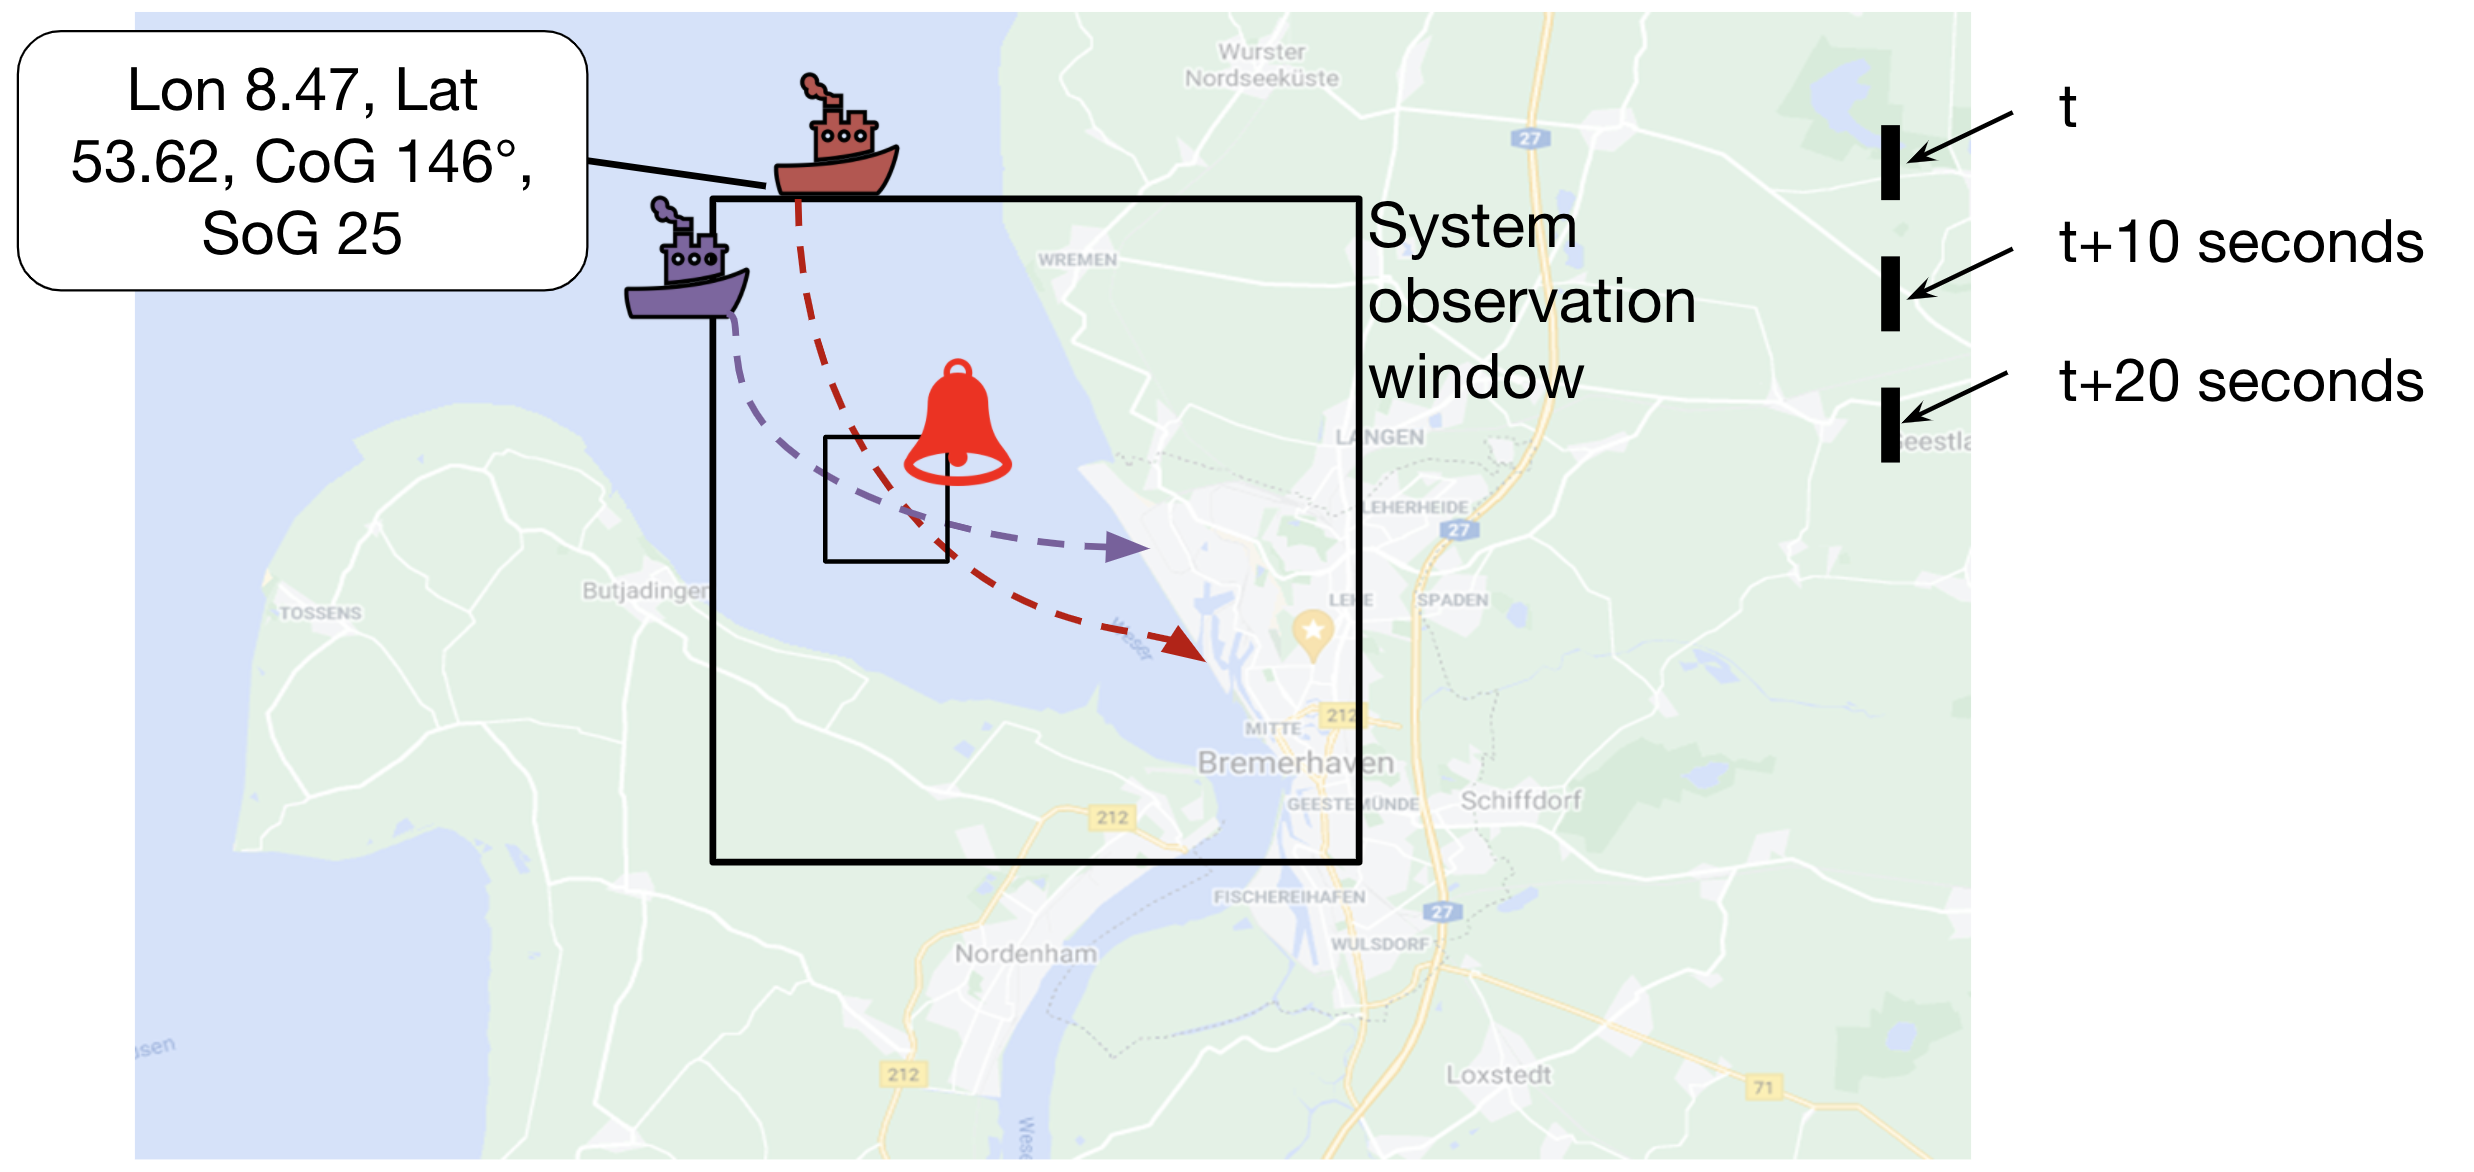
\includegraphics[width=\textwidth]{images/system_observation.png}
    \caption{System observation window}
    \label{fig:systemObservation}
\end{figure}